\documentclass{article}
\usepackage[letterpaper]{geometry}
\geometry{verbose,tmargin=1in,bmargin=1in,lmargin=1in,rmargin=1in}

\usepackage[utf8]{inputenc}
\usepackage{amsmath}
\usepackage{listings}
\usepackage{graphicx}
\usepackage{enumitem}

\title{CIS 419/519: Homework 1}
\author{\{Yupeng Li\}}
\date{}

\begin{document}
    \maketitle
    Although the solutions are entirely my own, I consulted with the following people and sources while working on this homework:
     \{http://www.cs.utep.edu/vladik/cs5315.13/cs5315\_13kader.pdf\}
    
    \section{Decision Tree Learning}
        \begin{enumerate}[label=\alph*.]
            \item % a
            Show your work:
            \begin{equation*}
                \mathit{InfoGain}(\mathit{PainLocation}) = \mathit{Info(X)- Info(X | PainLocation)} 
            \end{equation*}
	    \[\mathit{Info(X) = -\frac{9}{14} \log_2 \frac{9}{14} - \frac{5}{14} \log_2 \frac{5}{14} = 0.9402}\]
	    \[\mathit{InfoGain(PainLocation) = Info(X) - \frac{5}{14} (-\frac{3}{5} \log_2 \frac{3}{5} - \frac{2}{5} \log_2 \frac{2}{5}) - \frac{5}{14} (-\frac{2}{5} \log_2 \frac{2}{5} - \frac{3}{5} \log_2 \frac{3}{5})-0 = 0.2467}\]
		
            \begin{equation*}
                \mathit{InfoGain}(\mathit{Temperature}) =\mathit{Info(X) - Info(X | Temperature)}
            \end{equation*}
            \[\mathit{= Info(X) - \frac{4}{14} (-\frac{2}{4} \log_2 \frac{2}{4} - \frac{2}{4} \log_2 \frac{2}{4}) - \frac{10}{14} (-\frac{7}{10} \log_2 \frac{7}{10} - \frac{3}{10} \log_2 \frac{3}{10}) = 0.02499}\] 
            
            
            \item % b
            Show your work:
            \[\mathit{SplitInformation(PainLocation) = -\frac{5}{14} \log_2 \frac{5}{14} -\frac{5}{14} \log_2 \frac{5}{14} - \frac{4}{14} \log_2 \frac{4}{14} = 1.5774}\]
            \begin{equation*}
                \mathit{GainRatio}(\mathit{PainLocation}) = \mathit{\frac{InfoGain(PainLocation)}{SplitInformation(PainLocation)}} = \mathit{\frac{0.2467}{1.5774}} = \mathit{0.156397}
            \end{equation*}
             \[\mathit{SplitInformation(Temperature) = -\frac{4}{14} \log_2 \frac{4}{14} -\frac{10}{14} \log_2 \frac{10}{14}  = 0.86312}\]
            \begin{equation*}
                \mathit{GainRatio}(\mathit{Temperature}) = \mathit{\frac{InfoGain(Temperature)}{SplitInformation(Temperature)}} = \mathit{\frac{0.02499}{0.86312}} = \mathit{0.028953}
            \end{equation*}
            
            \item % c 
            ~\\
            
            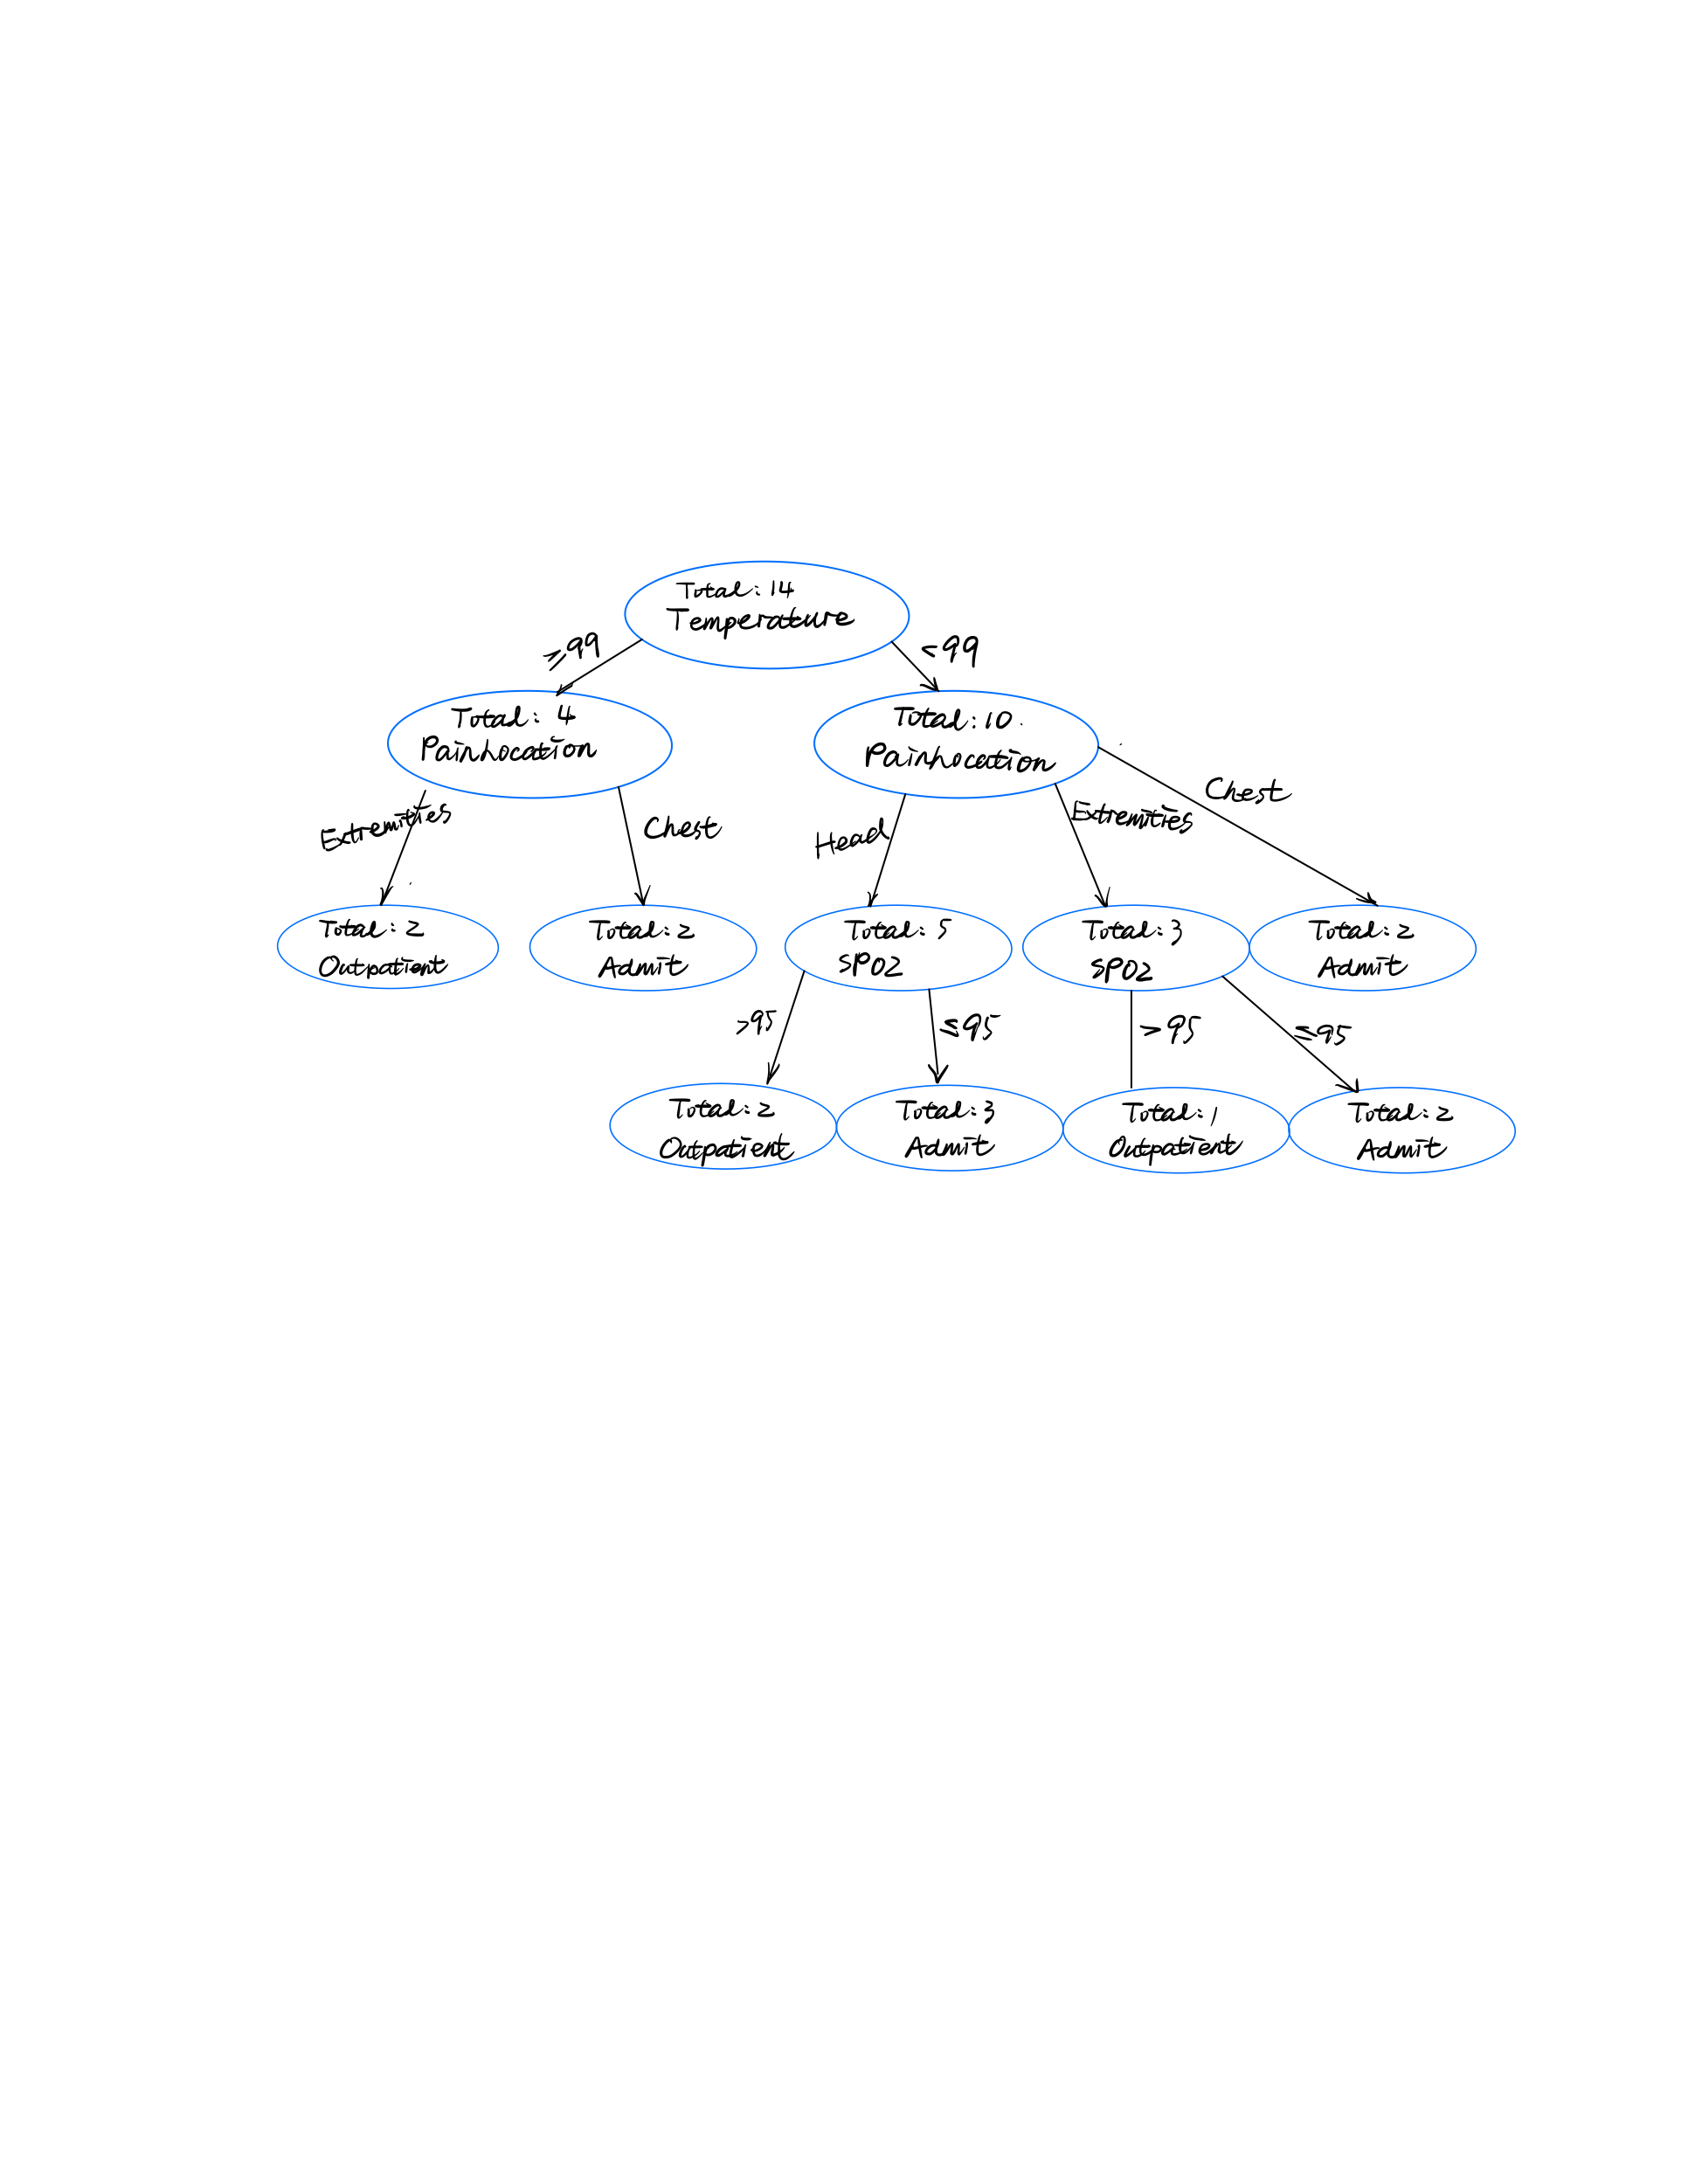
\includegraphics[width=0.8\textwidth]{HW1_Graph1}
                        
            \item % d
            No because finding the global optimal decision tree is NP hard  which has been proved in May, 1976. The advantage of ID3 is that it uses greedy approach which turns out to be really fast. ID3 will not produce the optimal decision tree, however, it gives good enough approximation. For more that 50\% of the datasets, ID3 can give the optimal solution.
        \end{enumerate}
        
       \section{Decision Trees \& Linear Discriminants [CIS 519 ONLY]}
        
        A decision tree can include oblique splits by...
        
        
        \section{Programming Exercises}
        \textbf{Features}: What features did you choose and how did you preprocess them?
        
        \noindent\textbf{Parameters}: What parameters did you use to train your best decision tree
        
        \noindent\textbf{Performance Table}: 
        \begin{center}
            \begin{tabular}{|c|c|c|}
                \hline
                Feature Set & Accuracy & Conf. Interval [519 ONLY]\\
                \hline
                DT 1 & a & b  \\
                DT 2 & a & b  \\
                DT 3 & a & b  \\
                \hline
        \end{tabular}
                \end{center}
        
        
        
        \textbf{Conclusion}: What can you conclude from your experience?
        
\end{document}